%%%%%%%%%%%%%%%%%%%%%%%%%%%%%%%%%%%%%%%%%%%%%%%%%%%%%%%%%%%%%%%%%%%%%%%%%%%%%%%
\section{Supplementary verification for the time-integrator comparison}
%%%%%%%%%%%%%%%%%%%%%%%%%%%%%%%%%%%%%%%%%%%%%%%%%%%%%%%%%%%%%%%%%%%%%%%%%%%%%%%

This section records implementation and convergence details supporting
Section~\ref{sec:time-integrators}.  The two-stage and three-stage
Gauss--Legendre methods were implemented by solving their coupled stage systems
with Newton iteration.  Exact tangent and adjoint actions were obtained by
linearizing the converged stage equations rather than by finite differences.

For a localized random edge perturbation $z$, we compared the tangent action
$Pz$ with
\begin{equation}
 \frac{\mathcal P_{\rm NL}(U_*+\delta z)
       -\mathcal P_{\rm NL}(U_*-\delta z)}{2\delta}.
\end{equation}
The minimum relative discrepancies before roundoff amplification were
$3.2\times10^{-5}$, $1.2\times10^{-4}$, and $1.3\times10^{-4}$ for midpoint,
GL4, and GL6.  The first-order-like asymptotic behavior near compacton zeros is
consistent with the map being $C^1$ but not $C^2$ there.  The adjoint identity
\begin{equation}
 \langle Pz,w\rangle=\langle z,P^*w\rangle
\end{equation}
was satisfied with relative discrepancies below $2.8\times10^{-14}$ for all
three methods.

\begin{figure}[t]
 \centering
 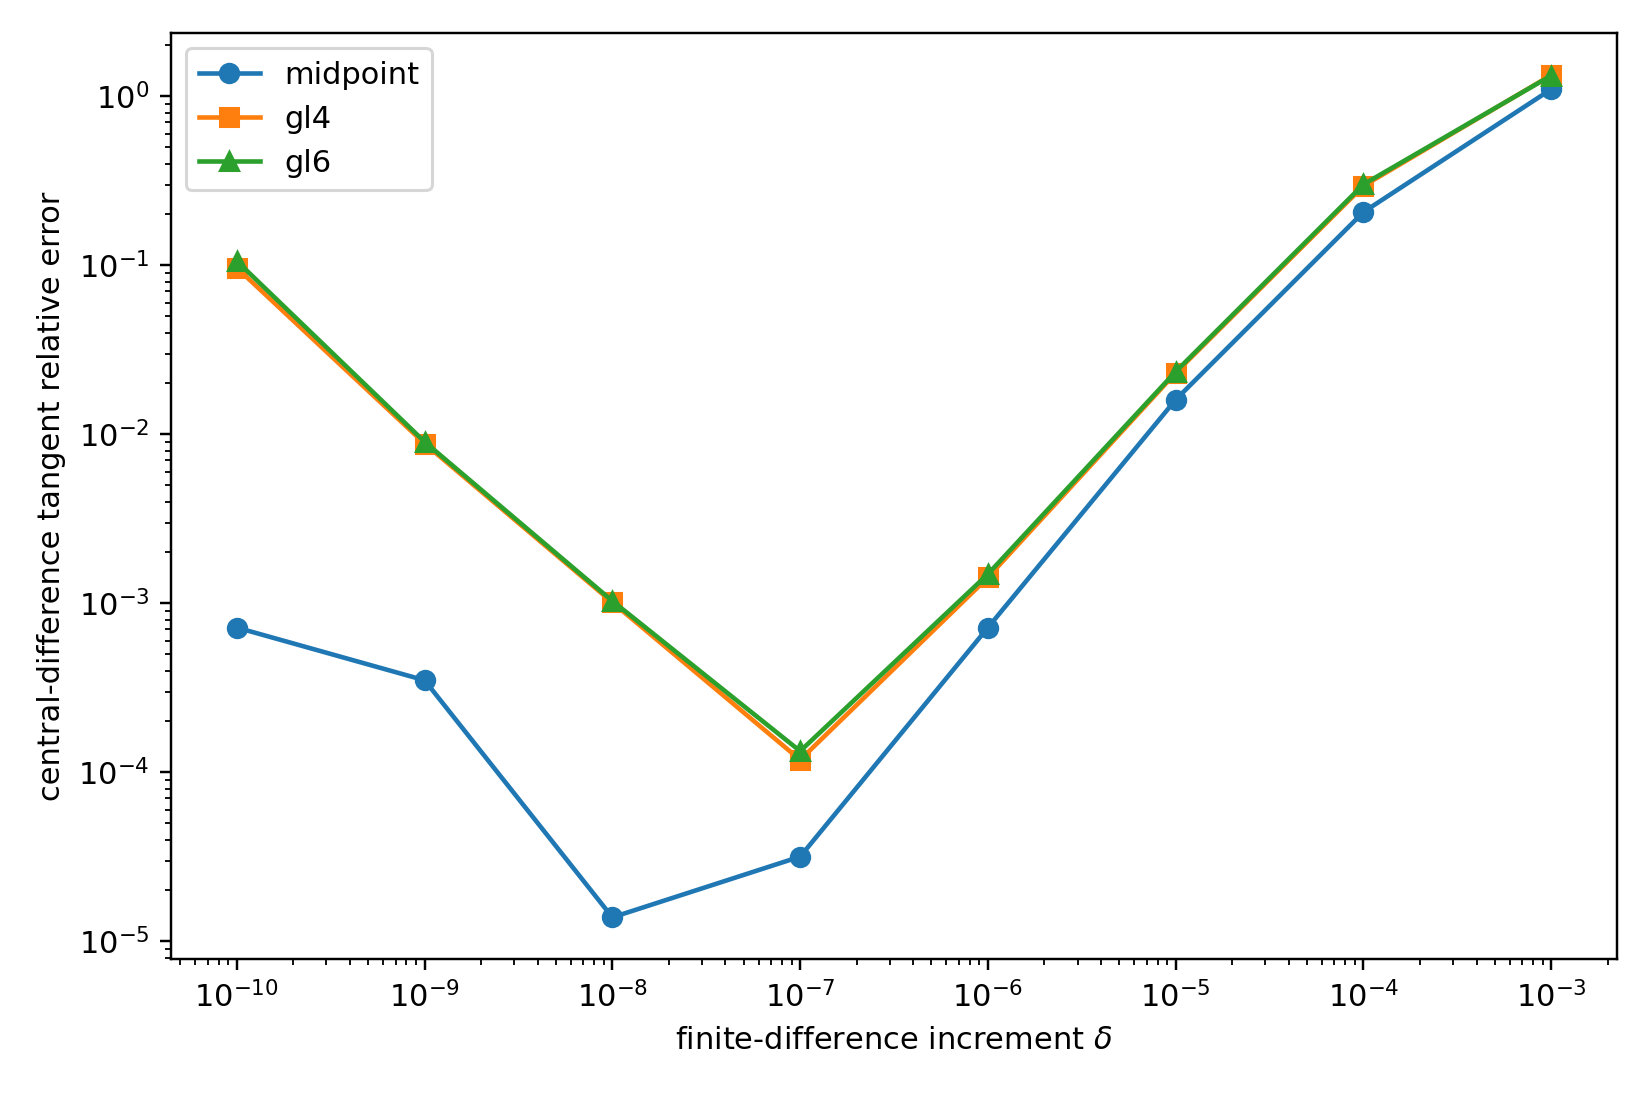
\includegraphics[width=0.70\textwidth]{wp3_tangent_directional_verification.png}
 \caption{Directional-derivative verification of the exact one-cell tangent
 maps for the three time integrators.}
\end{figure}

Independent GL4/GL6 reference ensembles give
\begin{equation}
 \rho_{F,\rm ref}=1.0958938054\pm8.9\times10^{-7}
 \quad(h=0.01),
\end{equation}
\begin{equation}
 \rho_{F,\rm ref}=1.1342141857\pm3.0\times10^{-7}
 \quad(h=0.02),
\end{equation}
where the quoted uncertainty is the half range of GL4 at
$\kappa=40,80$ and GL6 at $\kappa=10,20$.  It is an ensemble consistency
measure, not a probabilistic confidence interval.

A short exploratory natural GL6 calculation at $h=0.01$, $\kappa=5$ produced a
strong mixed forward high-frequency field but no isolated fixed-profile packet
within $t\le6$.  It was therefore excluded from the quantitative velocity
validation.  Its data and analysis scripts are retained in the reproducibility
archive.
%%%%%%%%%%%%%%%%%%%%%%%%%%%%%%%%%%%%%%%%%%%%%%%%%%%%%%%%%%%%%%%%%%%%%%%%%%%%%%%
